\subsection{实验环境搭建}
为香橙派开发板插上TYPEC电源适配器并用USB转TTL模块连接开发板与主机,连接完成后使用MobaXterm访问开发板,
终端连接WIFI成功如图:
\begin{figure}[H]
    \centering
    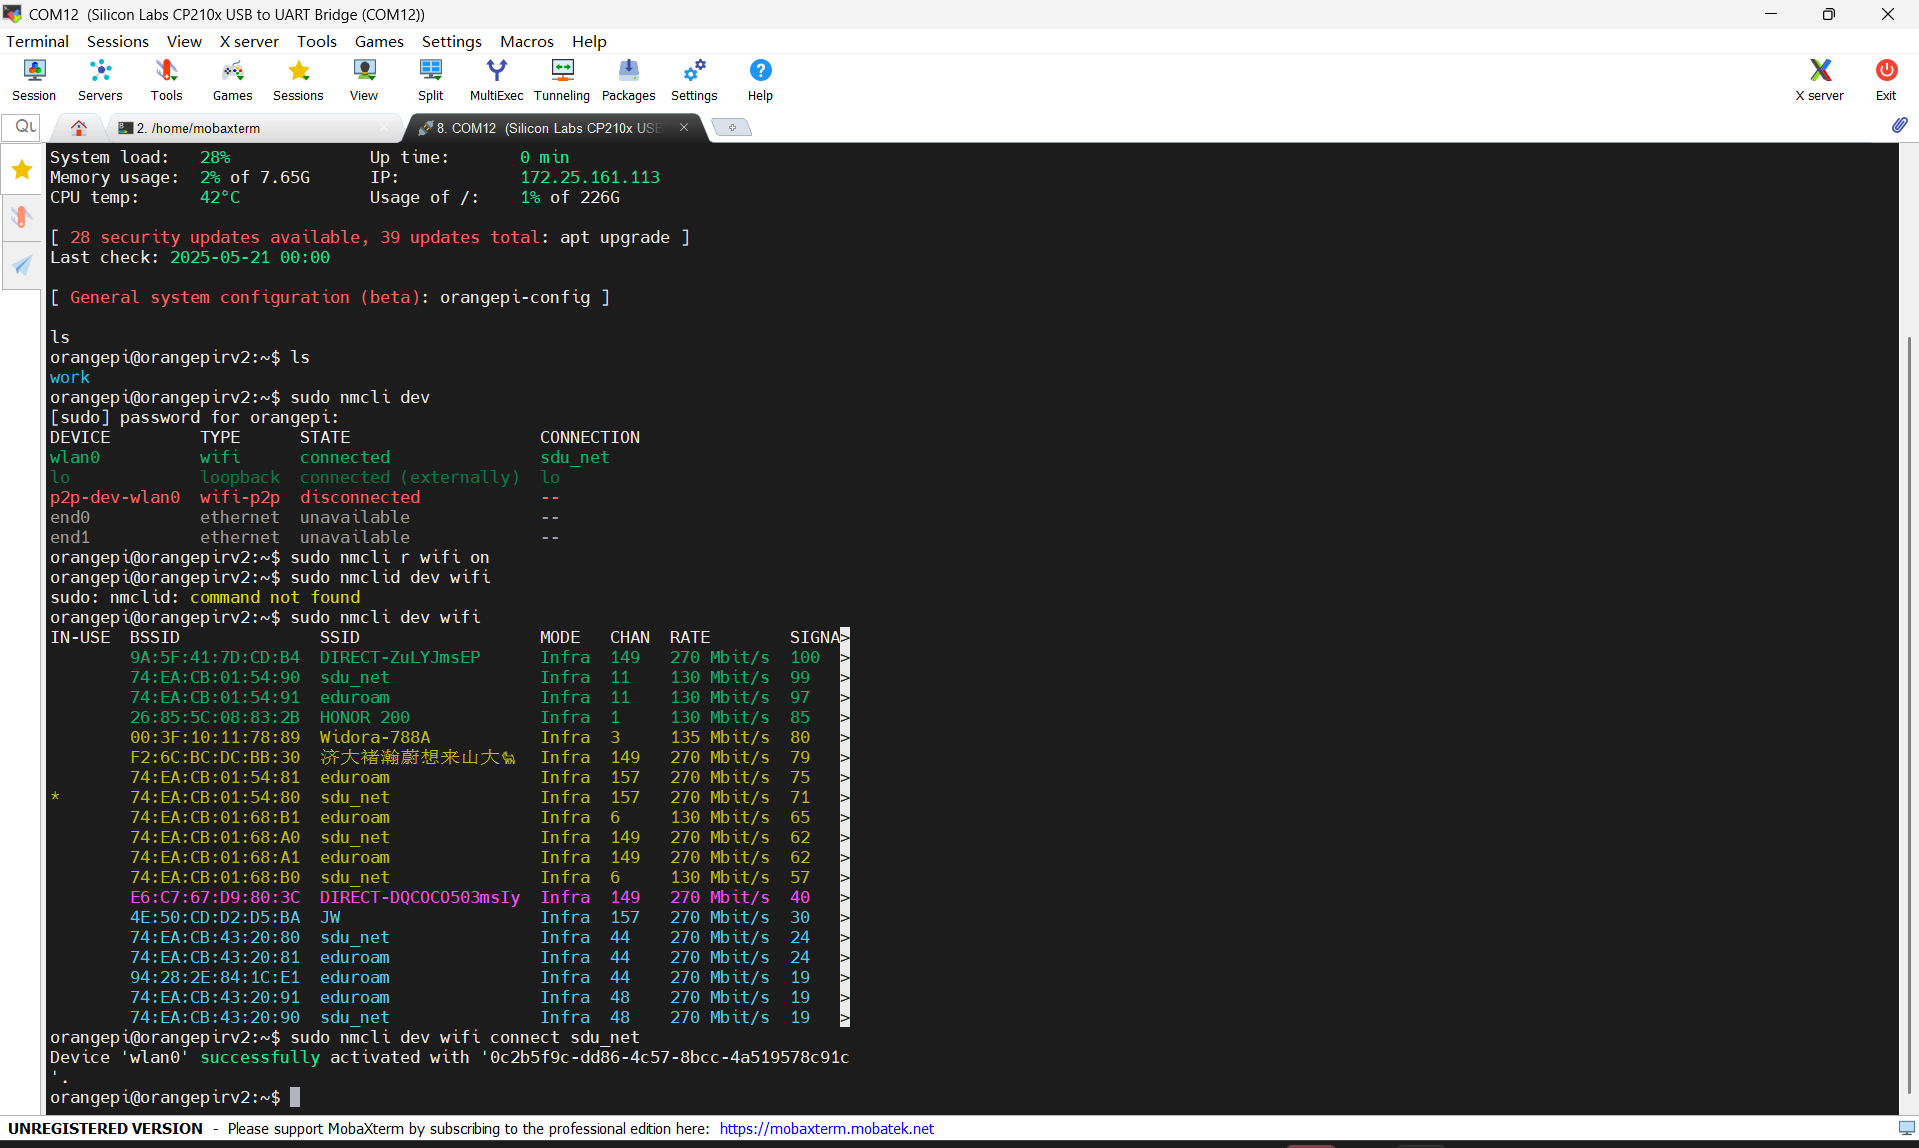
\includegraphics[width = 1\textwidth]{figure/conect_wifi.png}
    \caption{开发板连接WIFI}
\end{figure}
考虑到原实验为串口连接开发板进行单人次实验,而实际实验小组有多人,轮流使用串口会显著增加实验总耗时,不方便调试,也
不便于课后小组成员随时随地使用开发板的需要,因此我们为开发板配置网络后启动了OpenSSH服务。
基本实现为借助Tailscale工具将包括开发板在内的所有主机添加到同一个虚拟局域网中,使得所有设备都可以跨局域网登录访问开发板:
\begin{figure}[H]
    \centering
    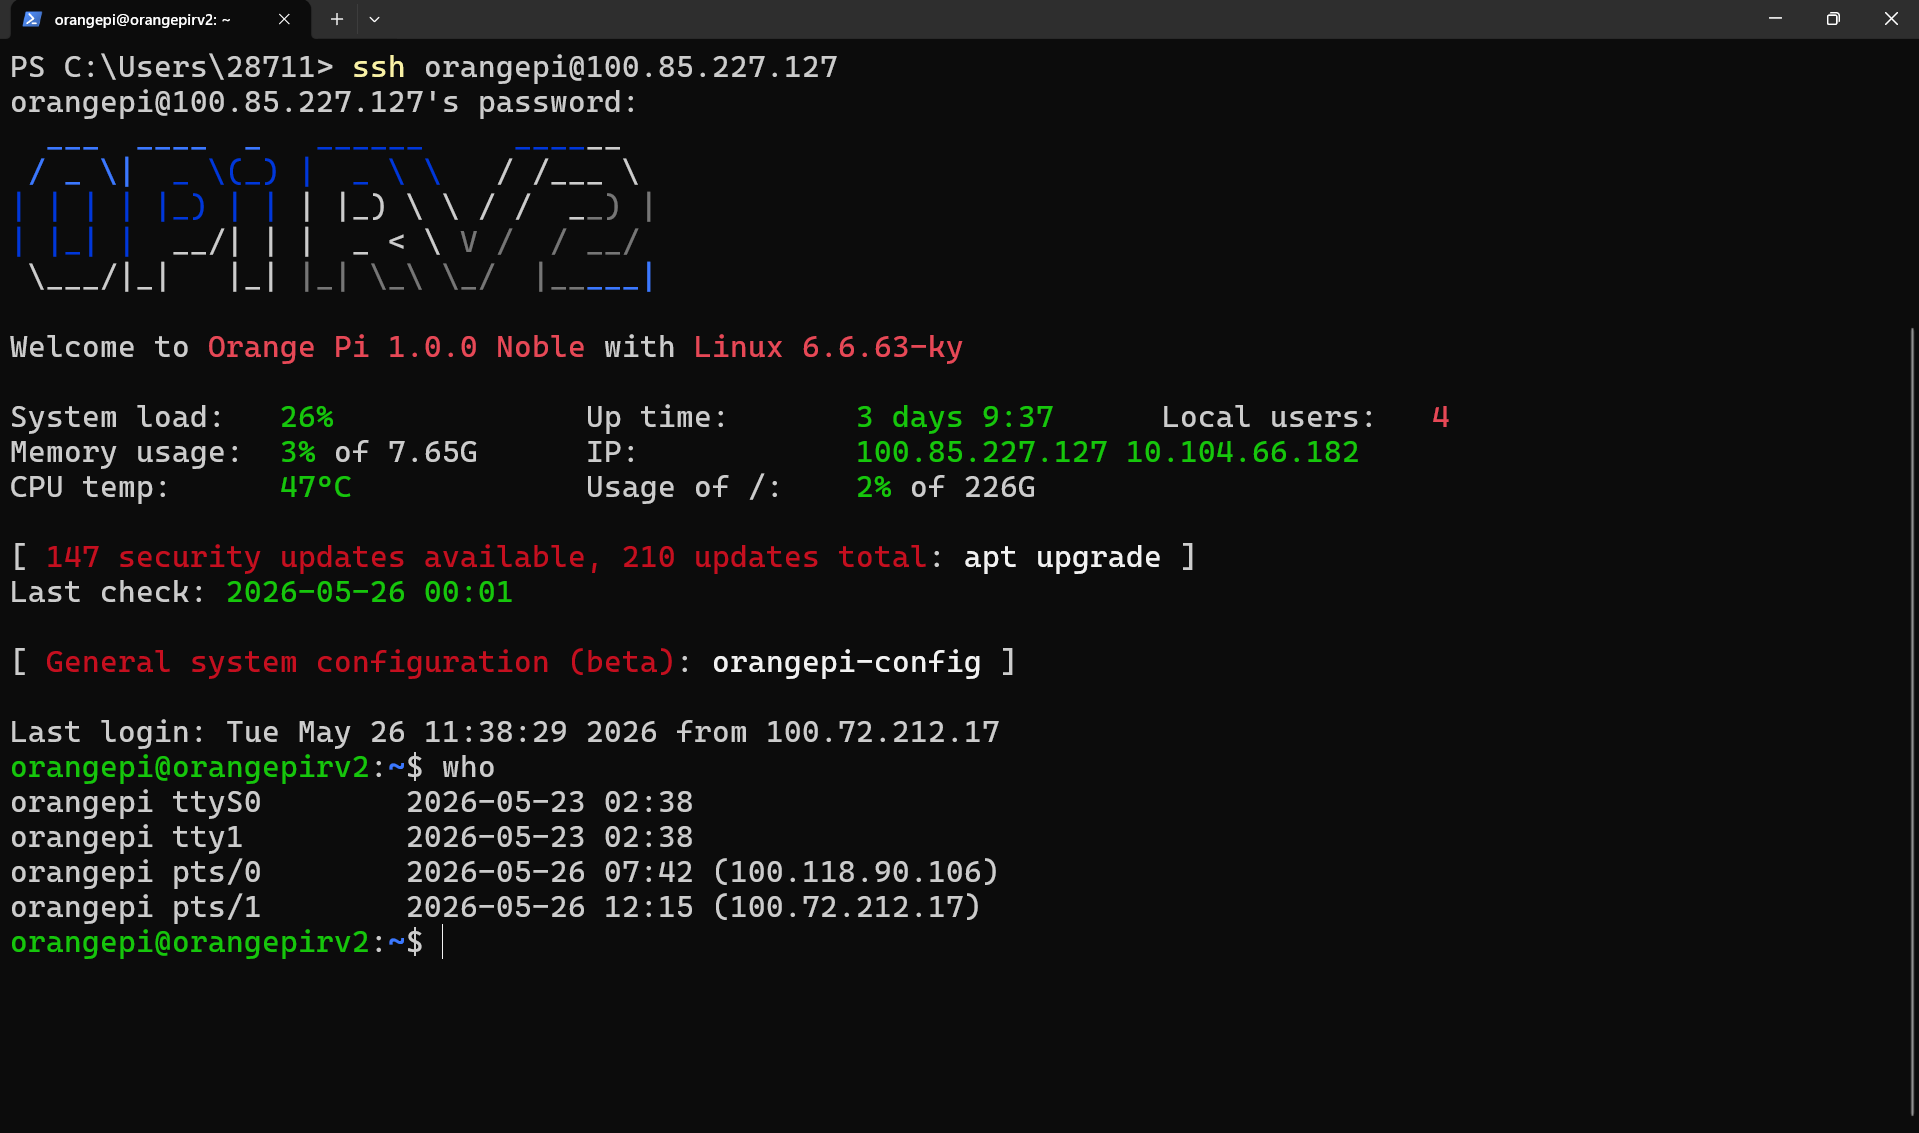
\includegraphics[width = 1\textwidth]{figure/ssh_sign_in.png}
    \caption{远程连接开发板}
\end{figure}
这里远程连接只是为了方便多用户远程访问开发板和编写代码,为确保实验结果准确性,每次测试算法效率时仅一位用户在使用。



